\chapter{Introduction}\label{ch:intro}


Human health and environmental quality are deeply linked. According to
the World Health Organization (WHO), in 2022 alone, at least 1.7 billion people
relied on contaminated drinking water sources, leading to an estimated 1 million
deaths from diarrhea. Additionally, ambient air pollution has emerged as the
leading environmental health risk, contributing to over 8 million deaths
annually \cite{air-pollution-mortality}. Addressing these challenges requires
data-driven decision-making. Yet, comprehensively modeling the complex physical
processes that drive changes in water and air quality at scales relevant to
human interactions is often computationally infeasible.

Despite this challenge, the environmental data volumes continues to expand
rapidly. For example, remote sensing platforms like Sentinel-2 generate
terabytes of multi-spectral imagery each day \cite{sentinel-2-data}. Next
generation systems, such as NASA’s recently launched PACE mission,
employ hyperspectral imagers capable of sampling \textit{hundreds} of individual
wavelength bands. At the same time, advancements in air quality measurement
technologies have led to a proliferation of new, low-cost sensors. Dense
networks of these sensors are being deployed across many urban areas to provide
real-time assessment of air quality dynamics. This wealth of data presents a
significant opportunity to inform environmental policy, with machine learning
techniques serving as a the primary tool to bridge the gap between our current
physical models and environmental data.




\section{Water Quality}

Water quality consists of the physical, chemical, and biological characteristics
of water, which characterize overall ecosystem health and its suitability for
uses such as drinking and agriculture. Poor water quality can result from a
range of anthropogenic and natural factors. Industrial pollution, particularly
from chemical manufacturing, mining, and agriculture, introduces
contaminants such as heavy metals, pesticides, and effluents into water
bodies \cite{schwarzenbach-water-pollution}. Urban runoff
picks up additional oils, plastics, and sediments, carrying them into
water sources where they cause a variety of issues such as
eutrophication and oxygen depletion \cite{smith-eutrophication}.
In addition to human activities, natural factors like soil erosion, volcanic
eruptions, and the leaching of naturally occurring metals from geological
formations can degrade water quality \cite{water-quality-natural}. Climate
change also plays a role, where increased water temperatures and altered
precipitation patterns contribute to the growth of harmful algal blooms
\cite{climate-change-water-quality}.

In situ and laboratory methods remain fundamental for water quality assessment,
providing direct and precise measurements for a variety of parameters. In situ
techniques involve the deployment of sensors and
instruments directly into water bodies to measure parameters such as pH,
dissolved oxygen, conductivity, and temperature. These sensors,
typically placed in monitoring stations or attached to buoys, often provide continuous
data streams essential for tracking short-term changes and local variability
\cite{in-situ-water-quality}. Portable instruments, such as multiparameter probes, are
also commonly used for spot measurements during field surveys, offering
flexibility in data collection across diverse environments. On the other hand,
laboratory analysis involves the collection of water samples which are then
transported to the lab for detailed examination.
Techniques such as mass spectrometry and liquid chromatography are used to
analyze heavy metals, pesticides, and organic compounds at
trace levels \cite{mass-spec-water, lc-ms}. Microbiological testing for harmful
pathogens is also used for assessing water safety, particularly for drinking
water \cite{microbio-methods}.

Despite their accuracy, in situ sampling and laboratory analysis suffer from
limited spatial coverage; the obtained measurements are only valid at the sample
site and are rarely representative of the spatial distributions of water quality
parameters. To enable parameter estimation over large bodies of water, remote sensing
techniques can be employed to relate observed radiometric properties to
optically active  water quality indicators such as turbidity, chlorophyll a, and
total suspended sediments \cite{remote-sensing-wq}. These optically active parameters
scatter and absorb ambient light according to their unique physical and chemical
properties. However, due to the limited wavelength bands of most remote sensing platforms
combined with incomplete prior knowledge of all components present a water body,
directly modeling the radiative transfer process to infer water quality
parameters is futile. Instead, empirical models for wavelength bands and
spectral indices are used to map remote sensing imagery to parameters of interest.
For example, Brezonik et al. successfully fit regression models to estimate
chlorophyll a and turbidity using band ratios from Landsat imagery \cite{brezonik-wq}.

The accuracy of water quality estimation using remote sensing data is
\textit{severely} constrained by the availability of coincident in situ
observations needed to train and validate empirical models. Because this method
relies on cloud-free satellite passes over fixed sensing sites, the data
curation process can require \textit{years} of observations to generate a few
thousand data points. For example, Aurin et al. combined measurements from
over 500 oceanographic field campaigns with over 30 years of coincident
satellite imagery to model CDOM absorption coefficients and CDOM
spectral slope \cite{aurin2018remote}. Similarly, Ross et al assembled
observations from 35 years of Landsat imagery with coincident measurements for
suspended sediment, CDOM, chlorophyl a, and Secchi disk depth (a measure of
water transparency) to facilitate model development for inland water quality.
These lengthy time scales curb analysis to historical trends and limiting
actionable insights during abrupt water quality crises such as oil spills
\cite{fingas2017review}.



\section{Air Quality}

Air quality refers to the composition of the atmosphere and its impact on human
health, ecosystems, and climate. The key components of air quality include
particulate matter (PM), ground-level ozone (\ce{O3}), nitrogen dioxide (\ce{NO2}), sulfur
dioxide (\ce{SO2}), carbon monoxide (\ce{CO}), and volatile organic compounds (VOCs).
Particulate matter refers to solid particles and liquid droplets suspended in
the air. PM is categorized according to its aerodynamic diameter as shown in
Figure~\ref{fig:pm-size-scale}, with \textit{fine} particulate matter
specifically referring to all particulates with a diameter below 2.5 microns (PM
2.5). PM originates from both natural sources, such as wildfires, dust storms, and
volcanic activity, as well as human activities, including vehicle emissions,
industrial processes, and the burning of fossil fuels \cite{pm-sources-1,
  air-chem-and-physics}. Ground-level ozone is a major component of smog
which forms when pollutants like \ce{NO2} and VOCs react in the presence of
sunlight and can cause respiratory problems and exacerbate conditions like
asthma \cite{ozone-health}. Nitrogen dioxide and sulfur dioxide primarily result
from the combustion of fossil fuels and are linked to respiratory inflammation
and acid rain \cite{no2-health, aq-and-health}.

\begin{figure}[!h]
  \centering
  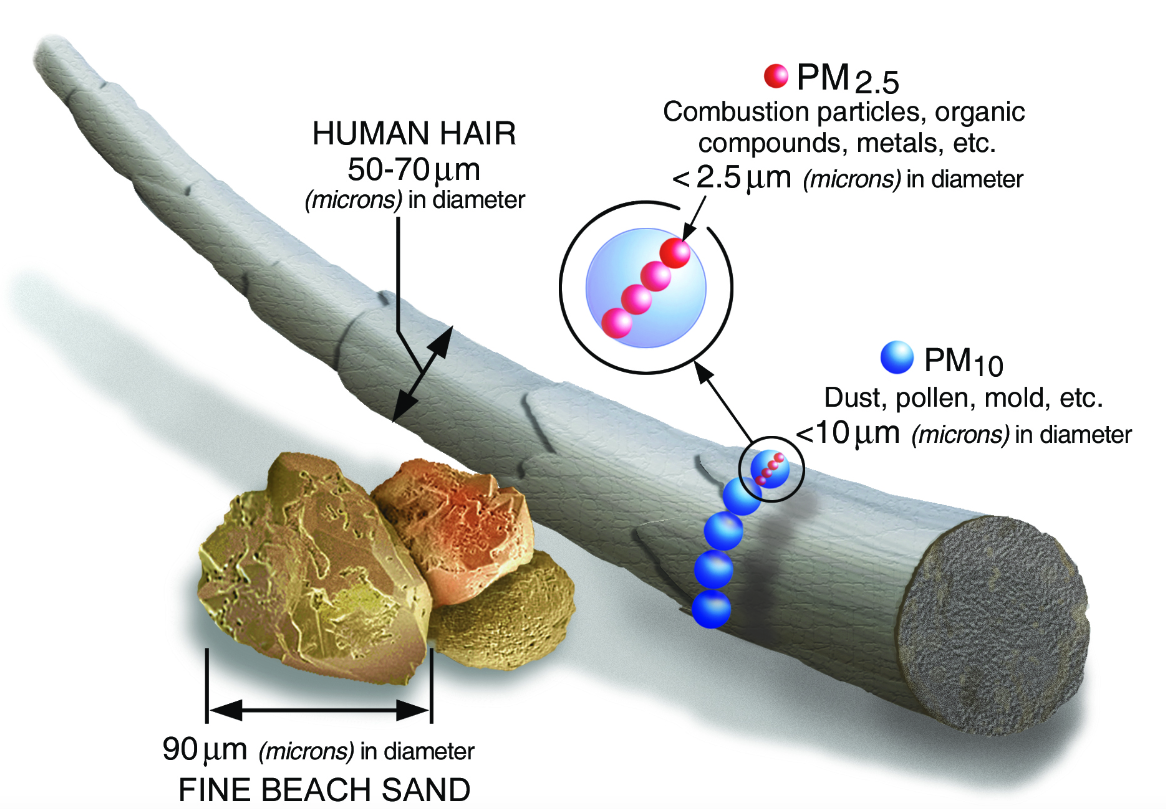
\includegraphics[width=0.75\columnwidth]{introduction/pm-size.png}
  \caption{Size comparisons for PM particles. Image source: US EPA
    (\url{https://www.epa.gov/pm-pollution/particulate-matter-pm-basics}, last
    accessed 2024-09-12).}
  \label{fig:pm-size-scale}
\end{figure}

PM is considered the most important air quality component due to its direct and
widespread impact on public health. Inhaled PM accumulates in the lungs, causing
both short-term and long-term health effects. Fine particulate matter,
specifically PM 2.5, is small enough to pass through the lungs and into the
bloodstream, increasing the risk of cardiovascular diseases, strokes, and cancer
\cite{pm-disease-1, pm-disease-2, pm-cancer}. Due to these combined effects, PM
exposure is estimated to be responsible for millions of premature deaths each
year \cite{pm-mortality-1, pm-mortality-fine}.

In response, many regulatory bodies have introduced new legislation explicitly aimed
at reducing PM levels. The European Union recently revised its air quality
standards to adopt a $10$ $\mu g/m^3$ annual limit for average PM 2.5.
The United States Environmental Protection Agency (EPA) has also adopted tighter
PM regulations, revising its annual PM 2.5 standard to $9$ $\mu g/m^3$ while
maintaining the $35$ $\mu g/m^3$ 24-hour limit.
These developments underscore the growing recognition of the threat posed by PM.


Annual and 24-hour PM regulations are designed to manage long-term exposure but
fail to capture acute spikes from short-term pollution events. These
transient PM spikes can lead to immediate increases in blood pressure, placing
vulnerable populations at heightened risk \cite{pm-bp}. Additionally, short-term
PM exposure has been shown to impair cognitive performance \cite{pm-cognition}.
In fact, the effects of PM on the body are strong enough that short-term PM 2.5
exposure can be independently estimated from a small assortment of biometric
sensors \cite{shawhin-biometrics, shisir-biometrics}. Therefore, high-resolution
PM data are essential for accurately quantifying the immediate impacts of local
PM pollution and facilitating timely mitigation efforts.

\section{Dissertation Goals}

The goal of this dissertation is to advance physical sensing in service of
society by leveraging physically motivated machine learning methods to extract
actionable insights from environmental data. Most modern machine learning models
are designed to solve \textit{general} learning tasks, such as image
classification and language prediction, for which the underly data may come
from a variety of sources with no representation in the real world.
In contrast to these abstract datasets, measurements from physical sensing systems
are governed by physical laws. This requirement imposes a strong constraint on
the space of possible model architectures; the predictions made
for environmental systems must be interpretable in their physical context. We
therefore adopt a physics-based approach, by which we mean a machine learning
techniques which strike a balance between data-driven learning and domain-specific
knowledge. This includes
\begin{itemize}
\item \textbf{Physically motivated model selection}: The chosen model should
  align with the underlying physical principles of the system under study. For
  example, a model predicting particulate matter should not allow for
  negative concentrations. Similarly, model assumptions for the underlying data
  distribution should apply to the measurement data.
\item \textbf{Integration of Prior Physical Knowledge}: Features corresponding
  to relevant physical quantities should be incorporated to improve model
  predictions. For example, the illumination geometry over a water body can
  significantly impact remote sensing imagery, and by extension, the
  estimation of water quality parameters.
\item \textbf{Interpretability}: Understanding \textit{how} a model makes
  predictions is just as important as prediction accuracy. Preference should be
  given to models with explainable structures. Additionally, the quantification of
  model uncertainty is vital for making informed decisions.
\end{itemize}
Towards this end, this work presents a collection of case studies utilizing both
supervised and unsupervised machine learning techniques for the assessment of
water quality and air quality.

In the first category, we are focused on answering the basic question:
\textit{Is this water safe?}. Localized in situ measurements for specific water
quality parameters do not provide sufficient spatial coverage to assess water
quality across water bodies with variable topography, composition, and flow. Remote
sensing imagery can cover far wider areas, but simple empirical models
insufficient to robustly map complex spectra to contaminant concentrations. We
therefore utilize machine learning to bridge this gap.

For air quality measurement, our goal is to develop predictive models which can
resolve abrupt pollution spikes in PM time series while \textit{also} enabling
short-term forecasts. Many complicated machine learning models have been
developed for generic time series analysis. In this work, we focus on developing
physically-motivated models based on known PM dynamics. As secondary goal, these
models should be small enough to be deployable on low-cost sensing hardware.


\section{Research Contributions}

The research presented in this manuscript involved the collection of multiple
datasets \textit{and} the creation of software for data processing, modeling,
and analysis. The studies presented in Chapters~\ref{ch:robot-team-supervised}
and \ref{ch:robot-team-gtm} have been published in peer-reviewed journals. The
study from Chapter~\ref{ch:robot-team-gsm} is currently in review, and a
manuscript for the study presented in Chapter~\ref{ch:havok} is in preparation.
A comprehensive list of these various contributions is provided below in
Table~\ref{tab:contributions}


\begin{table}[H]
  \caption{Datasets, software, and publications developed for this dissertation.}
  \label{tab:contributions}
  \begin{center}
    \resizebox{\textwidth}{!}{\begin{tabular}{lccc} \hline
      \textbf{Title} & \textbf{Type} & \textbf{Chapter(s)} & \textbf{Status} \\ \hline
      Autonomous Learning of New Environments with a Robotic Team & & & \\
      Employing Hyper-Spectral Remote Sensing, Comprehensive In-Situ & Article & \ref{ch:robot-team} & published, \cite{robot-team-1}  \\
      Sensing and Machine Learning & & & \\ \hline
      Characterizing Water Composition With an Autonomous Robotic & & & \\
      Team Employing Comprehensive in Situ Sensing, Hyperspectral & Article & \ref{ch:robot-team-supervised} & published, \cite{robot-team-2} \\
      Imaging, Machine Learning, and Conformal Prediction & & & \\ \hline
      Unsupervised Characterization of Water Composition With & & & \\
      Uav-Based Hyperspectral Imaging and Generative Topographic & Article & \ref{ch:robot-team-gtm} & published, \cite{robot-team-gtm} \\
      Mapping & & & \\ \hline
      Generative Simplex Mapping: & & & \\
      Non-linear Endmember Extraction & Article & \ref{ch:robot-team-gsm} & Submitted, In Review \\
      and Spectral Unmixing for Hyperspectral Imagery & & & \\ \hline
      Interpretable Time-delay Embedding Models & & & \\
      for Low-Cost Particulate Matter Sensors: & Article & \ref{ch:havok} & In Preparation \\
      Forecasting and Outlier Detection & & & \\ \hline
      & & & \\
      \texttt{RobotTeam.jl} & Code & \ref{ch:robot-team}, \ref{ch:robot-team-supervised}, \ref{ch:robot-team-gtm}, \ref{ch:robot-team-gsm} & \href{https://github.com/john-waczak/RobotTeam.jl}{Julia Package} \\
      & & & \\ \hline
      & & & \\
      \texttt{SolarGeometry.jl} & Code & \ref{ch:robot-team-supervised} & \href{https://github.com/john-waczak/SolarGeometry.jl}{published, Julia Package} \\
      & & & \\ \hline
      & & & \\
      \texttt{GenerativeTopographicMapping.jl} & Code & \ref{ch:robot-team-gtm}, \ref{ch:robot-team-gsm} & \href{https://github.com/john-waczak/GenerativeTopographicMapping.jl}{published, Julia Package} \\
      & & & \\ \hline
      & & & \\
      \texttt{MLJNonnegativeMatrixFactorization.jl} & Code & \ref{ch:robot-team-gsm} & \href{https://github.com/john-waczak/MLJNonnegativeMatrixFactorization.jl}{published, Julia Package} \\
      & & & \\ \hline
      & & & \\
      HAVOK time series models & Code & \ref{ch:havok} & \href{https://github.com/john-waczak/aq-havok.jl}{Code repository} \\
      & & & \\ \hline

      & & & \\
      Live Air Quality Dashboards & (live) Data & \ref{ch:air-network} & \href{http://mdash.circ.utdallas.edu:3000}{Website} \\
      & & & \\ \hline
      & & & \\
      Air Quality Database & Dataset & \ref{ch:air-network},\ref{ch:havok} & \href{http://mdash.circ.utdallas.edu:8086}{Website} \\
      & & & \\ \hline
      & & & \\
      Robot team Hyperspectral Images & Dataset & \ref{ch:robot-team-supervised}, \ref{ch:robot-team-gtm}, \ref{ch:robot-team-gsm} & \href{https://ncsa.oxn.xsede.org/ees230012-bucket01}{OSN S3 Bucket} \\
      & & & \\ \hline
      & & & \\
      MINTS Air Network Historical Data  & Dataset & \ref{ch:air-network} & \href{https://ncsa.oxn.xsede.org/ees230012-bucket01}{OSN S3 Bucket} \\
      & & & \\ \hline
    \end{tabular}}
  \end{center}
\end{table}



\section{Dissertation Overview}

In Chapter~\ref{ch:robot-team} we first provide a general overview of the
interaction between light and water which motivates the use of hyperspectral imaging
for the assessment of water quality and composition. We then describe a
autonomous robotic team developed to coordinate drone-based hyperspectral imaging
with in situ data collection to greatly accelerate the data acquisition process
for water quality studies. We provide a detailed description of the
georeferencing and reflectance conversion procedures developed to process
hyperspectral images and conclude with an evaluation of total image processing times.

Next, in Chapter~\ref{ch:air-network} we outline measurement techniques for
particulate matter sensing before describing a low-cost network of distributed
air quality monitors designed to collect real-time PM data. We then describe a
containerized data pipeline combining multiple open-source tools to process
network data, provide live visualization dashboards, and enable redundant
data storage.

In Chapter~\ref{ch:robot-team-supervised} we develop a family of supervised
machine learning models to map reflectance spectra to key water composition
parameters. Importantly, this approach utilizes conformal prediction
to assess distribution-free confidence intervals for model predictions. We
examine the relative importance of model features to identify key wavelength
bins for each target variable. Each model is then applied to map the
distributions of physical, chemical, ionic, and biochemical parameters across a
North Texas Pond.

In Chapter~\ref{ch:robot-team-gtm} we expand the capabilities of the robot team
to address situations for which water contaminants are not known in advance. In
this scenario, ground-truth data are not available, and therefore, unsupervised
machine learning methods are needed to identify sources using only hyperspectral
images. We utilize Generative Topographic Mapping for this task and demonstrate
it's ability to visualize the spatial distribution of reflectance spectra across
the water. A rhodamine tracer die released into the pond is then used to
demonstrate that this unsupervised approach successfully identifies unique
spectral signatures which can be used to map contaminant dispersion.

Next, in Chapter~\ref{ch:robot-team-gsm} we present a novel, physics-based
method for unsupervised spectral unmixing and endmember extraction.
This approach builds on the latent variable structure of Generative Topographic
Mapping to directly model linear and nonlinear mixing of radiometric data.
The model is evaluated against Non-negative Matrix Factorization for a
synthetic dataset of mixed spectra from the USGS spectral database. We then
apply the method to unmix water-based hyperspectral images captured by the robot
team. The same rhodamine dye is used to test the ability of the method to map
the dispersion of unknown contaminants across the water.

In Chapter~\ref{ch:havok} we return to the air quality network in order to develop time
series models for local particulate matter data. Given that particulate matter
generally follows a diurnal cycle with intermittent pollution spikes, we
leverage the Hankel Alternative View of Koopman method to simultaneously model
PM time series \textit{and} extract these occasional spikes. We then utilize
this framework to develop short-term forecasting capabilities.

Finally, in Chapter~\ref{ch:future-work} we present directions for future work
before summarizing the conclusions for each study in
Chapter~\ref{ch:conclusions}.




% Big data in the physical sciences
% Comment on the annual data volumes produced by
% \begin{itemize}
%   \item LANDSAT
%   \item Sentinel
%   \item CERN
%   \item James Webb
%   \item SDO AIA
%   \item Medical Imaging (MRI, CT scans, etc...)
% \end{itemize}

% What is machine learning

% Use of machine learning in the physical sciences

% \begin{itemize}
%   \item Remote sensing (inter-instrument calibration, classification, object identification, change monitoring via the NDVI and similar indices, etc.)
%   \item Protein Folding
%   \item Drug discovery
%   \item Surrogate modeling (i.e. for PDE solvers - now very popular at NVIDIA)
% \end{itemize}


% \subsection{Supervised and Unsupervised ML}


% \subsection{Physics-based Machine Learning}



